
%(BEGIN_QUESTION)
% Copyright 2007, Tony R. Kuphaldt, released under the Creative Commons Attribution License (v 1.0)
% This means you may do almost anything with this work of mine, so long as you give me proper credit

One of the most basic water-treatment processes is {\it clarification}: letting the water move {\it slowly} through a large, open vessel for the purpose of allowing solids to precipitate.  The resulting ``clarified'' water will be less turbid than the incoming water, with the precipitate being collected out the bottom of the clarifier vessel as sludge:

$$\includegraphics[width=15.5cm]{i01807x01.eps}$$

\filbreak

When multiple clarifiers are used, it is common to operate each at the same flow rate: in other words, with the influent flow equally split between the multiple clarifiers.  Sketch a P\&ID for a control system that will match flow through clarifiers \#2 and \#3 at rates equal to the flow through clarifier \#1:

$$\includegraphics[width=15.5cm]{i01807x02.eps}$$

\vskip 20pt \vbox{\hrule \hbox{\strut \vrule{} {\bf Suggestions for Socratic discussion} \vrule} \hrule}

\begin{itemize}
\item{} A useful analytical technique for any complex control system is to annotate the diagram with ``+'' and ``-'' symbols at the instrument bubble inputs, designating ``noninverting'' and ``inverting'' characteristics, respectively.  Show how this helps you track of all directions of action, making it easier to figure out how the control system responds to changes.
\item{} For those who have studied flow measurement, explain what a {\it weir} is and how one works to measure water flow through an open channel.
\end{itemize}

\underbar{file i01807}
%(END_QUESTION)





%(BEGIN_ANSWER)

Here is a simple solution, using 1:1 ratio control to make the bottom and middle clarifiers match flow with the top clarifier:

$$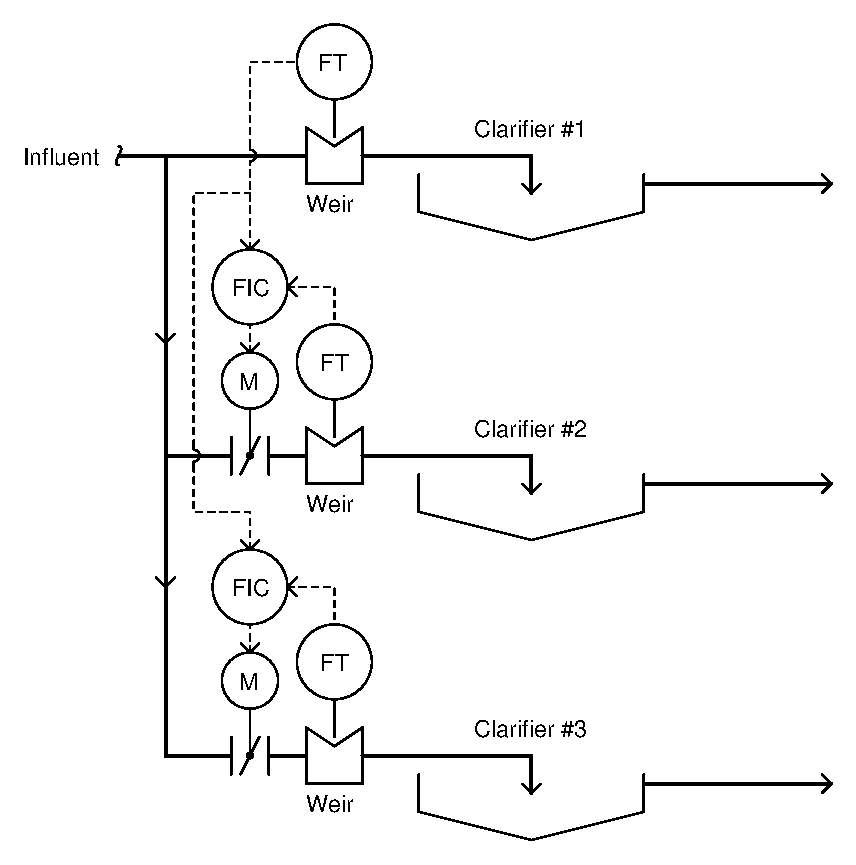
\includegraphics[width=15.5cm]{i01807x03.eps}$$

%(END_ANSWER)





%(BEGIN_NOTES)


%INDEX% Control, strategies: water clarifier flow balance control
%INDEX% Process: municipal water clarification

%(END_NOTES)


